\documentclass[border=10pt]{standalone}
\usepackage[svgnames]{xcolor}
\usepackage{amsmath}
\usepackage{pgfplots}
\pgfplotsset{compat=newest}
\usepackage[sfdefault]{FiraSans}
\usepackage{FiraMono}
\renewcommand*\familydefault{\sfdefault}
\begin{document}
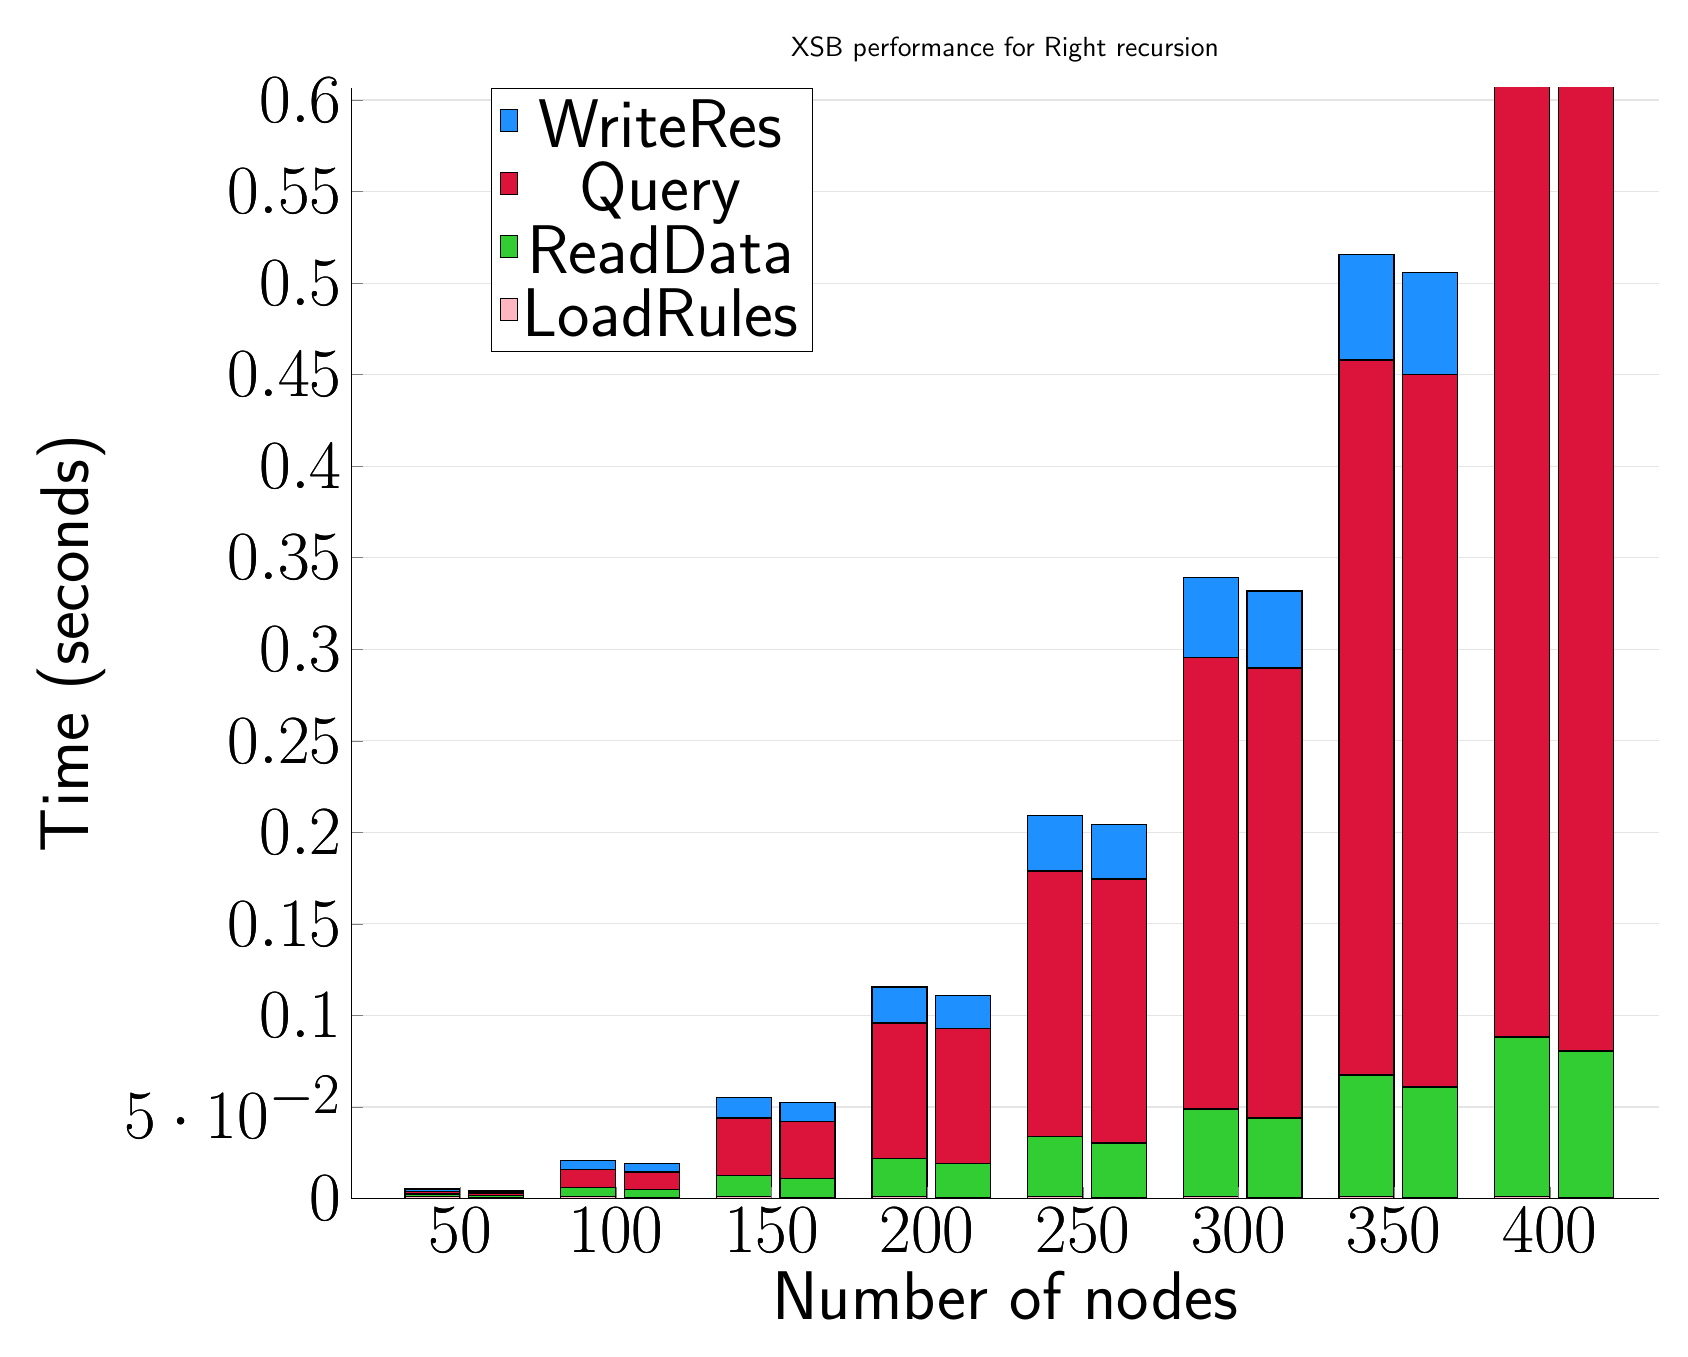
\begin{tikzpicture}
	\begin{axis}[
			ybar stacked,
			title={XSB performance for Right recursion},
			bar shift=-10pt,
			width=1.5\textwidth,
			bar width=0.7cm,
			ymajorgrids, tick align=inside,
			major grid style={draw=gray!20},
			xtick=data,
			ymin=0, ymax=0.6066430044174194,
			axis x line*=bottom,
			axis y line*=left,
			enlarge x limits=0.1,
			legend style={
					at={(0.23, 1)},
					anchor=north,
					legend columns=1,
					font=\Huge,
				},
			ylabel={Time (seconds)},
			xlabel={Number of nodes},
			label style={font=\Huge},
			tick label style={font=\Huge},
		]
		\addlegendimage{fill=DodgerBlue, draw=black, line width=0.2pt}
		\addlegendentry{WriteRes}
		\addlegendimage{fill=Crimson, draw=black, line width=0.2pt}
		\addlegendentry{Query}
		\addlegendimage{fill=LimeGreen, draw=black, line width=0.2pt}
		\addlegendentry{ReadData}
		\addlegendimage{fill=LightPink, draw=black, line width=0.2pt}
		\addlegendentry{LoadRules}
		\addplot +[fill=LightPink, draw=black, line width=0.5pt] coordinates {
				(50, 0.0010690927505493178)
				(100, 0.001052570343017579)
				(150, 0.001043581962585451)
				(200, 0.001066064834594726)
				(250, 0.001035213470458985)
				(300, 0.001050186157226562)
				(350, 0.0010905265808105482)
				(400, 0.00108015537261963)
			};
		\addplot +[fill=LimeGreen, draw=black, line width=0.5pt] coordinates {
				(50, 0.001524305343627929)
				(100, 0.0051391124725341806)
				(150, 0.01151936054229736)
				(200, 0.02070932388305665)
				(250, 0.03273375034332276)
				(300, 0.04778809547424316)
				(350, 0.06637849807739257)
				(400, 0.08718564510345458)
			};
		\addplot +[fill=Crimson, draw=black, line width=0.5pt] coordinates {
				(50, 0.0012936353683471683)
				(100, 0.009529185295104981)
				(150, 0.03145799636840819)
				(200, 0.07419049739837646)
				(250, 0.14504027366638178)
				(300, 0.24682199954986567)
				(350, 0.39059689044952395)
				(400, 0.5854477167129518)
			};
		\addplot +[fill=DodgerBlue, draw=black, line width=0.5pt] coordinates {
				(50, 0.001396656036376953)
				(100, 0.00513322353363036)
				(150, 0.01126332283020021)
				(200, 0.01960718631744384)
				(250, 0.030468916893005505)
				(300, 0.043583583831786996)
				(350, 0.05772852897644041)
				(400, 0.0728026390075682)
			};
	\end{axis}
	\begin{axis}[
			ybar stacked,
			bar shift=13pt,
			width=1.5\textwidth,
			bar width=0.7cm,
			ymajorgrids, tick align=inside,
			major grid style={draw=none},
			xtick=data,
			ymin=0, ymax=0.6066430044174194,
			axis x line*=none,
			axis y line*=none,
			enlarge x limits=0.1,
			label style={font=\Huge},
			tick label style={font=\Huge},
		]
		\addplot +[fill=LightPink, draw=black, line width=0.5pt] coordinates {
				(50, 0.0006271)
				(100, 0.0006166000000000004)
				(150, 0.0006108999999999996)
				(200, 0.0006007999999999996)
				(250, 0.0005962999999999998)
				(300, 0.0006098000000000001)
				(350, 0.0006278999999999996)
				(400, 0.0006121)
			};
		\addplot +[fill=LimeGreen, draw=black, line width=0.5pt] coordinates {
				(50, 0.0011819)
				(100, 0.0044548999999999995)
				(150, 0.0102316)
				(200, 0.0185252)
				(250, 0.029668099999999996)
				(300, 0.04331809999999999)
				(350, 0.060356900000000005)
				(400, 0.0799406)
			};
		\addplot +[fill=Crimson, draw=black, line width=0.5pt] coordinates {
				(50, 0.0012682000000000001)
				(100, 0.0094437)
				(150, 0.0312102)
				(200, 0.073782)
				(250, 0.1443604)
				(300, 0.24582600000000002)
				(350, 0.3891722)
				(400, 0.5827848)
			};
		\addplot +[fill=DodgerBlue, draw=black, line width=0.5pt] coordinates {
				(50, 0.0011434)
				(100, 0.004635599999999999)
				(150, 0.0104344)
				(200, 0.017969600000000002)
				(250, 0.029538999999999992)
				(300, 0.04214179999999999)
				(350, 0.0556636)
				(400, 0.07121339999999997)
			};
	\end{axis}
\end{tikzpicture}

\end{document}
